\documentclass{article}
\usepackage{inputenc}
\usepackage{setspace}
\usepackage[margin=0.75in]{geometry}
\usepackage[style=numeric]{biblatex}
\addbibresource{ref.bib}
\usepackage{float}
\usepackage{graphicx}
\graphicspath{ {./images/} }


\onehalfspace
\setlength{\parindent}{0pt}
\setlength{\parskip}{1em}



\begin{document}

\begin{center}
  \LARGE{\textbf{Real-world Functional Programming}} \\
  \Large{Project Report} \\
  \normalsize{14274056 Junsong Yang (psyjy3)} \\
  \today
\end{center}


\begin{normalsize}
  \section{Introduction}
  In this section, the general idea about this project will be introduced as
  well as how this project would fit for this module.

  The project is called recipe house, which is a recipe recommendation service based on the ingredients. The logic behind it is quite simple. It would require users to input whatever ingredients they have, then it will return recipes that used those ingredients. This project includes two parts: a back-end
  server and a web interface. Since I don't have any recipe database, the
  back-end server will query a third-party API for recipe info and trim the
  returned data in JSON and return the trimmed data as a response to the web
  interface.

  The third-party APIs that I will use are provided by Edamam. They have over 2
  millions of recipes specified by diets, calories, nutrient ranges and simply
  just ingredients.

  This project idea was used to compete in ATOS IT Challenge and was shortlisted(top 20 worldwide). The back-end was written in Go as well as the web interface with a bit vanilla javascript, but it was not quite finished.
  Hence, this idea will be reimplemented in a different approach for this
  project.

  As for how this project may fit for 10 credits:
  \begin{itemize}
  \item[]{learning scala for backend (about 20 hrs)}
  \item[]{learning React (with any host language) (20 hrs)}
  \item[]{revisit web technologies (HTML CSS) (10 hrs)}
  \item[]{implementation of the back-end (15 hrs)}
  \item[]{implementation of the web interface (15 hrs)}
  \item[]{report writing (20 hrs)}  
  \end{itemize}

  A successful project would be a working web interface that allowed the user to use either text-based or image-based search for recipes based on what ingredients they have. The front-end would send the ingredients info to the back-end
  server via REST API. Then the back-end server will query the third-party API
  for recipes and parse the returned data and sent back to the front-end as a response. The front-end will present the response from the server to the end-user. 


  \section{Technical Background}
  In this section, the technological choices made for both the back end and
  the front end will be discussed in detail with justification.

  For the backend server, the language of choice is Scala. Scala is a multi-paradigm
  programming language compiles to java bytecode and supports both functional programming and imperative programming. Hence, by using scala, we can not only explore functional programming in-depth but also leveraging the java ecosystem. The backend server provides service through REST APIs, therefore,
  the play framework is chosen to serve this purpose. The play framework supports MVC architecture by default, but this project is not designed that way. The project does not include database and the frontend is implemented separately. Hence, only controllers will be created.

  As for the frontend interface, a javascript library called React will be used.
  The reason for that choice is that React supports functional reactive
  programming paradigm which can be used to create a graphical user interface.
  Functional reactive programming is a programming paradigm that been studied over the years and there are a few attempts to apply functional reactive programming to graphical user interface designs. React is not purely functional by nature as it relies on javascript as its underlying programming language. But the design decisions made for this library are inspired by functional reactive programming. Hence, React can be used to design a graphical user interface using
  functional reactive programming.
  
  \section{Implementation}
  In this section, the general architecture of this project will be introduced
  as well as some essential implementation details.

  \subsection{Architecture}
  \begin{figure}[H]
    \centeringng
    \centerline{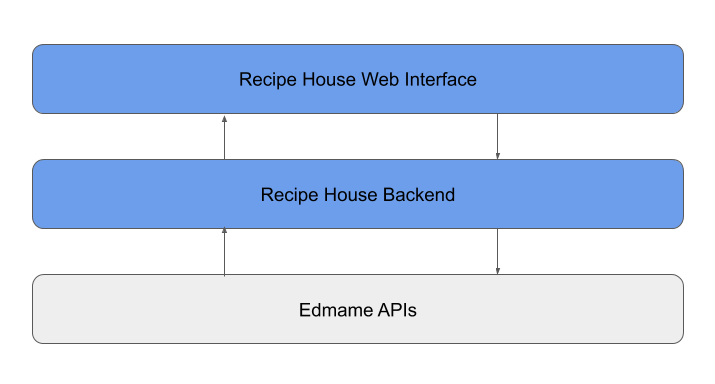
\includegraphics[scale=0.4]{archi}}
    \caption{Architecture of this project}
    \label{fig:architecture}
  \end{figure}

  Figure \ref{fig:architecture} shows the overall structure of this project.
  This project mainly consists of two parts. The recipe house web interface and backend server. The web interface provides access to end-users. The name of ingredients can be input through the web interface. The web interface will requests the backend server accordingly for recipe data then those data will be presented to the end-user through the web interface. As for the backend server, It provides services to the web interface through REST APIs. Given the input from the user, the backend server will query the edamame API for recipe information. 

  \subsection{Backend}
  \begin{figure}[H]
    \centeringng
    \centerline{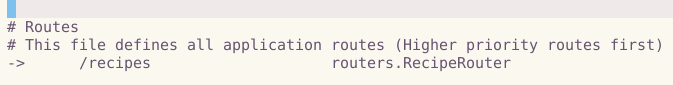
\includegraphics[scale=0.8]{route}}
    \caption{Architecture of this project}
    \label{fig:route}
  \end{figure}
  The backend server is implemented using play framework. Figure \ref{fig:route}
  shows the contains of the route file. The arrow suggested that this route is
  defined generically. Any route that matches the route defined above will be
  handled by the RecipeRouter in routers package.

  \begin{figure}[H]
    \centeringng
    \centerline{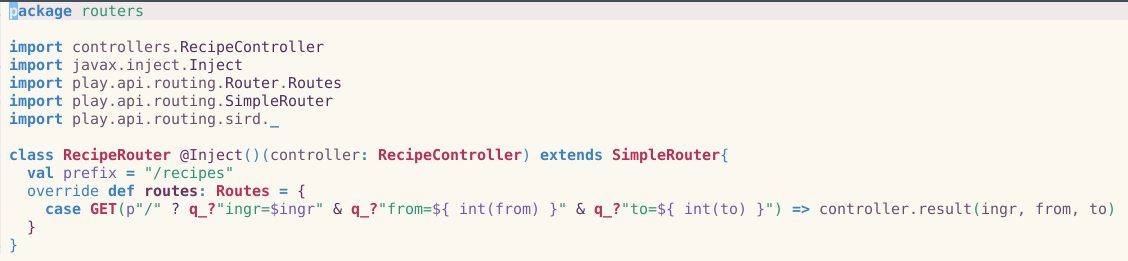
\includegraphics[scale=0.6]{router}}
    \caption{Architecture of this project}
    \label{fig:router}
  \end{figure}
  Figure \ref{fig:router} depicted the implementation of the router. The route here is defined using pattern matching and domain-specific language provided by the play framework. This domain-specific language will strip the parameters
  inside the URL and then pass to the result function defined in the
  RecipeController. As shown in figure \ref{fig:router}, the ingr, from and to is passed the result function. Specifically, the data types of those parameters need to be mentioned here. They are normal data types wrapped in a
  datatype called Option. The Option type is equivalent to the Maybe monad in
  Haskell, it either has a value or nothing.
  

  \begin{figure}[H]
    \centeringng
    \centerline{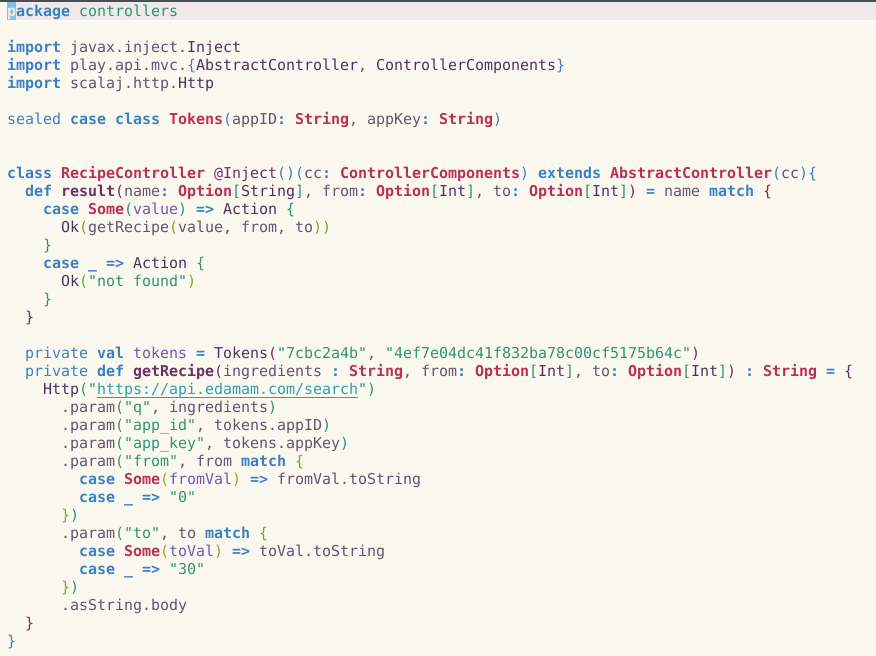
\includegraphics[scale=0.7]{controller}}
    \caption{Architecture of this project}
    \label{fig:controller}
  \end{figure}
  Figure \ref{fig:controller} shows the implementation of the RecipeController.
  This controller has two functions, the result function and the getRecipe
  function. The result function will first do the pattern matching on the name parameter as it contains the ingredients' name. If the name parameter contains some value, then the getRecipe function will be called. Otherwise, the result function will just return not found.

  As for the getRecipe function, it takes three parameters, ingredients, from and to. The from and to parameters are wrapped in Option data type as they are optional. The getRecipe function will query edamam API as return the response
  as a result.

  To store the credentials for querying the edamam API, a case class was created. The case class is a built-in Scala feature that can be used to
  modelling immutable data.

  \subsection{Frontend}
    \begin{figure}[H]
    \begin{minipage}[b]{0.48\linewidth}
      \centering
      \centerline{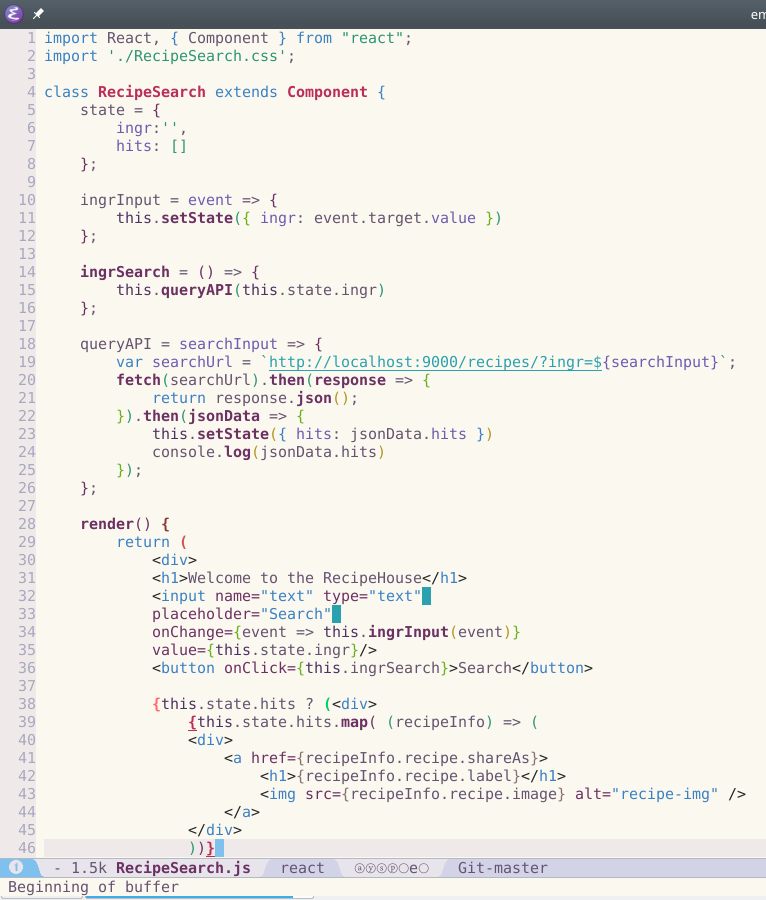
\includegraphics[width=8.5cm, height=10cm]{react1}}
      \centerline{ (a) Web Interface Part I}\medskip
    \end{minipage}
    \hfill
    \begin{minipage}[b]{0.48\linewidth}
      \centering
      \centerline{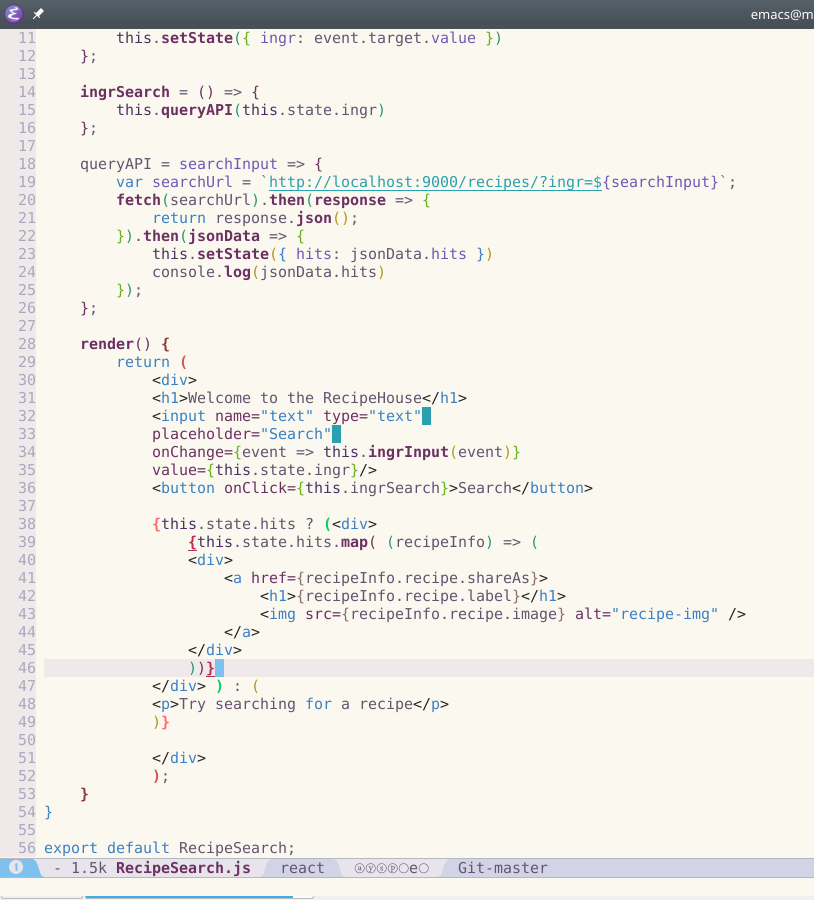
\includegraphics[width=8.5cm, height=10cm]{react2}}
      \centerline{ (b) Web Interface Part II }\medskip
    \end{minipage}
    \caption{Recipe House Web Interface}
    \label{fig:react}
  \end{figure}

  The web interface of this project is implemented using React. Figure
  \ref{fig:react} shows how the recipe search component was implemented. Many concepts in React were inspired by functional programming including React components. Components in React are immutable which means once they cannot be changed directly once they are defined. To cope with this situation, a tuple called state is created to store data that may change according to different events.

  The ingrInput is an arrow function to obtain the user input from the input box and store the input into the state tuple. Followed by ingrSearch, which is an
  arrow function to call the queryAPI function when the search button is
  clicked and store the returned recipe data into the state tuple.

  The last part is the render function. This function will print all the UI
  components like buttons and input box on the screen. The UI components are defined using a domain-specific language called JSX. The last part of the render function is the display of recipes. The state tuple will be checked first to determine whether there were any recipe data or not. If recipe data is already presented in the state tuple then they will be displayed.
  
  \section{Reflection}
  Functional programming started drawing attention over the last few years.
  Ideas and concepts of functional programming are absorbed by a vast array of imperative languages but the adoption rate of the functional programming language is still negligible. Functional programming is a solution to many problems but it is not a silver bullet as the world is running imperatively. Compare
  to backend development, functional programming is more acceptable for frontend
  development as javascript is aggressively adopting functional programming
  features. Additionally, libraries like React is inspired and influenced by
  functional programming which increased the exposure of functional programming
  to frontend developer.

  There are reasons that language like Haskell is rarely adopted by industries compare to other imperative languages like Java. For someone who comes from the imperative background without prior knowledge of functional programming, it is quite hard to grasp concepts the way Haskell presents them. But for me, since
  I am comfortable with Haskell in general, I found Scala is quite familiar and more accessible. For the functional programming paradigm, Haskell and Scala shared the same foundation, hence, they support similar features but in different ways. The Scala way is a bit different but quite acceptable. With the support of imperative programming, Scala is more applicable to the real-world scenarios than Haskell.
  
\end{document}
